% ============================================================
%  PathOptLearn — Research Presentation
%  Beamer + TikZ  |  pdflatex
% ============================================================
\documentclass[aspectratio=169,12pt]{beamer}

% ── Theme ────────────────────────────────────────────────────
\usetheme{Madrid}
\usecolortheme{default}
\definecolor{primary}{RGB}{25,80,160}
\definecolor{accent}{RGB}{230,80,30}
\definecolor{lightgray}{RGB}{245,245,248}
\definecolor{darkgray}{RGB}{60,60,70}
\definecolor{codeblue}{RGB}{0,100,180}
\definecolor{codegreen}{RGB}{0,130,80}
\definecolor{codeorange}{RGB}{200,100,0}

\setbeamercolor{palette primary}{bg=primary,fg=white}
\setbeamercolor{palette secondary}{bg=primary!80,fg=white}
\setbeamercolor{palette tertiary}{bg=primary!60,fg=white}
\setbeamercolor{frametitle}{bg=primary,fg=white}
\setbeamercolor{title}{fg=white}
\setbeamercolor{block title}{bg=primary,fg=white}
\setbeamercolor{block body}{bg=lightgray,fg=darkgray}
\setbeamercolor{alerted text}{fg=accent}
\setbeamercolor{structure}{fg=primary}

% ── Packages ─────────────────────────────────────────────────
\usepackage[utf8]{inputenc}
\usepackage[T1]{fontenc}
\usepackage{lmodern}
\usepackage{tikz}
\usepackage{pgfplots}
\pgfplotsset{compat=1.18}
\usetikzlibrary{arrows.meta,shapes.geometric,positioning,fit,
                backgrounds,calc,decorations.pathreplacing,matrix}
\usepackage{booktabs}
\usepackage{multirow}
\usepackage{listings}
\usepackage{amsmath,amssymb}
\usepackage{fontawesome5}
\usepackage{xcolor}
\usepackage{graphicx}
\usepackage{hyperref}

% ── Code style ───────────────────────────────────────────────
\lstdefinestyle{code}{
  basicstyle=\ttfamily\scriptsize,
  keywordstyle=\color{codeblue}\bfseries,
  commentstyle=\color{codegreen},
  stringstyle=\color{codeorange},
  backgroundcolor=\color{lightgray},
  frame=single,framerule=0.4pt,
  rulecolor=\color{primary!30},
  breaklines=true,
  tabsize=2,
  showstringspaces=false,
}
\lstset{style=code}

% ── Slide numbering ──────────────────────────────────────────
\setbeamertemplate{footline}{%
  \leavevmode%
  \hbox{\begin{beamercolorbox}[wd=.33\paperwidth,ht=2.25ex,dp=1ex,left,leftskip=1em]
    {author in head/foot}\usebeamerfont{author in head/foot}PathOptLearn\end{beamercolorbox}%
  \begin{beamercolorbox}[wd=.34\paperwidth,ht=2.25ex,dp=1ex,center]
    {title in head/foot}\usebeamerfont{title in head/foot}
    Adaptive Learning Platform\end{beamercolorbox}%
  \begin{beamercolorbox}[wd=.33\paperwidth,ht=2.25ex,dp=1ex,right,rightskip=1em]
    {date in head/foot}\usebeamerfont{date in head/foot}
    \insertframenumber{} / \inserttotalframenumber\end{beamercolorbox}}%
  \vskip0pt}
\setbeamertemplate{navigation symbols}{}

% ── TikZ helpers ─────────────────────────────────────────────
\tikzset{
  box/.style={rectangle,rounded corners=4pt,draw=primary,
              fill=lightgray,text width=#1,align=center,
              minimum height=1cm,font=\small},
  box/.default=2.6cm,
  arrow/.style={-Stealth,thick,primary},
  dbarrow/.style={-Stealth,thick,accent,dashed},
  node box/.style={rectangle,rounded corners=6pt,draw=primary!60,
                   fill=primary!8,minimum height=0.8cm,
                   align=center,font=\footnotesize,inner sep=4pt},
  db/.style={cylinder,shape border rotate=90,draw=primary,
             fill=primary!15,minimum height=1cm,minimum width=1.2cm,
             align=center,font=\tiny},
  badge/.style={circle,draw=accent,fill=accent!20,
                font=\scriptsize\bfseries,inner sep=2pt},
}

% ── Meta ─────────────────────────────────────────────────────
\title[PathOptLearn]{\textbf{PathOptLearn}\\[4pt]
  \large An Adaptive AI-Powered Learning Platform\\
  with Knowledge-Graph-Grounded Recommendations}
\subtitle{TER — Université Paris-Saclay}
\author{PathOptLearn Research Team}
\date{2026}
\institute{Université Paris-Saclay\\
           Département Informatique}

% ============================================================
\begin{document}
% ============================================================

% ── Title slide ──────────────────────────────────────────────
{
\setbeamertemplate{footline}{}
\begin{frame}[plain]
  \begin{tikzpicture}[remember picture,overlay]
    \fill[primary] (current page.north west) rectangle
        ([yshift=-3.2cm]current page.north east);
    \node[white,font=\Large\bfseries] at
        ([yshift=-1.1cm]current page.north)
        {PathOptLearn};
    \node[white,font=\normalsize] at
        ([yshift=-2.0cm]current page.north)
        {An Adaptive AI-Powered Learning Platform};
    \node[white!80,font=\small] at
        ([yshift=-2.6cm]current page.north)
        {with Knowledge-Graph-Grounded Recommendations};
  \end{tikzpicture}
  \vspace{3.5cm}
  \begin{columns}
    \column{0.5\textwidth}
      \textbf{TER — Université Paris-Saclay}\\[2pt]
      \small Département Informatique\\[6pt]
      \footnotesize 2026
    \column{0.5\textwidth}
      \raggedleft
      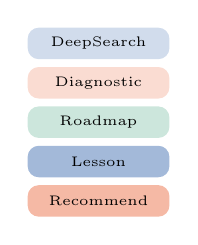
\begin{tikzpicture}
        \foreach \i/\c/\l in {0/primary!20/DeepSearch,
                               1/accent!20/Diagnostic,
                               2/codegreen!20/Roadmap,
                               3/primary!40/Lesson,
                               4/accent!40/Recommend}{
          \node[rectangle,rounded corners,fill=\c,
                font=\tiny,minimum width=1.8cm,
                minimum height=0.4cm] at (0,-\i*0.5) {\l};
        }
      \end{tikzpicture}
  \end{columns}
\end{frame}
}

% ── Outline ──────────────────────────────────────────────────
\begin{frame}{Outline}
  \tableofcontents
\end{frame}

% ============================================================
\section{Motivation \& Problem Statement}
% ============================================================

\begin{frame}{The Problem with Static Learning Paths}
  \begin{columns}
    \column{0.55\textwidth}
      \begin{block}{Limitations of current platforms}
        \begin{itemize}
          \item One-size-fits-all curriculum
          \item No assessment of prior knowledge
          \item Resources not matched to specific gaps
          \item No feedback loop between quizzes and content
        \end{itemize}
      \end{block}
      \vspace{6pt}
      \begin{alertblock}{Research Question}
        Can we build a system that \textbf{diagnoses} a learner's
        knowledge state, \textbf{searches} the open web for resources,
        and \textbf{adapts} the learning path dynamically?
      \end{alertblock}
    \column{0.42\textwidth}
      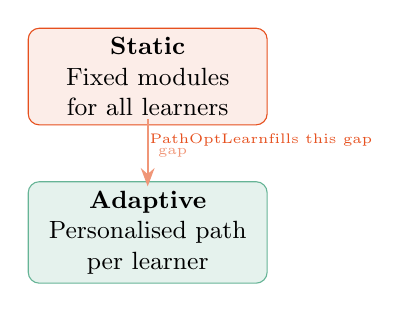
\begin{tikzpicture}[scale=0.9]
        % Static vs adaptive
        \node[box=2.8cm,fill=accent!10,draw=accent] at (0,2.2)
            {\textbf{Static}\\Fixed modules\\for all learners};
        \node[box=2.8cm,fill=codegreen!10,draw=codegreen!60] at (0,0)
            {\textbf{Adaptive}\\Personalised path\\per learner};
        \draw[-Stealth,thick,accent!60] (0,1.6) -- node[right,font=\tiny]{gap} (0,0.65);
        \node[font=\tiny,accent] at (1.6,1.3) {PathOptLearn\\fills this gap};
      \end{tikzpicture}
  \end{columns}
\end{frame}

% ============================================================
\section{System Architecture}
% ============================================================

\begin{frame}{High-Level Architecture}
  \begin{center}
  \begin{tikzpicture}[node distance=0.5cm and 1.0cm]

    % Frontend
    \node[rectangle,rounded corners=6pt,draw=codegreen!70,
          fill=codegreen!10,minimum width=2.2cm,
          minimum height=1.2cm,align=center,font=\small]
          (fe) {\faLaptop\\[2pt]\textbf{Streamlit}\\Frontend};

    % API
    \node[rectangle,rounded corners=6pt,draw=primary,
          fill=primary!10,minimum width=2.2cm,
          minimum height=1.2cm,align=center,font=\small,
          right=1.4cm of fe]
          (api) {\faCode\\[2pt]\textbf{FastAPI}\\Backend};

    % LLM
    \node[rectangle,rounded corners=6pt,draw=accent,
          fill=accent!10,minimum width=2.2cm,
          minimum height=1.0cm,align=center,font=\small,
          above=0.7cm of api]
          (llm) {\faBrain\\[2pt]\textbf{Ollama LLM}};

    % Postgres
    \node[db,right=1.4cm of api,yshift=0.7cm]
          (pg) {\faDatabase\\[2pt]PostgreSQL};

    % Neo4j
    \node[db,right=1.4cm of api,yshift=-0.7cm]
          (neo) {\faProjectDiagram\\[2pt]Neo4j KG};

    % Web
    \node[rectangle,rounded corners=4pt,draw=darkgray!60,
          fill=darkgray!8,minimum width=2.2cm,
          minimum height=0.8cm,align=center,font=\small,
          above=0.7cm of fe]
          (web) {\faGlobe\ Web / YouTube};

    % Arrows
    \draw[arrow] (fe) -- (api);
    \draw[arrow] (api) -- (llm);
    \draw[arrow] (api) -- (pg);
    \draw[arrow] (api) -- (neo);
    \draw[dbarrow] (web) -- (api);

    % Labels
    \node[font=\tiny,primary] at ($(fe)!0.5!(api)+(0,-0.7)$)
        {REST + Streaming};
    \node[font=\tiny,accent] at ($(api)!0.5!(llm)+(0.6,0)$)
        {Prompts};
    \node[font=\tiny,primary] at ($(api)!0.5!(pg)+(0,0.2)$)
        {CRUD};
    \node[font=\tiny,primary] at ($(api)!0.5!(neo)+(0,-0.2)$)
        {Cypher};

  \end{tikzpicture}
  \end{center}
  \vspace{-4pt}
  \begin{columns}
    \column{0.33\textwidth}
      \centering\small \textcolor{codegreen}{\faCheck}\ Containerised (Docker Compose)
    \column{0.33\textwidth}
      \centering\small \textcolor{codegreen}{\faCheck}\ Fully offline-capable (Ollama)
    \column{0.33\textwidth}
      \centering\small \textcolor{codegreen}{\faCheck}\ Streaming responses
  \end{columns}
\end{frame}

% ── Technology stack ─────────────────────────────────────────
\begin{frame}{Technology Stack}
  \begin{columns}
    \column{0.5\textwidth}
      \begin{table}
        \centering\small
        \begin{tabular}{ll}
          \toprule
          \textbf{Layer} & \textbf{Technology} \\
          \midrule
          Frontend     & Streamlit 1.35 \\
          API          & FastAPI + Uvicorn \\
          LLM          & Ollama (\texttt{llama3.2:1b}) \\
          Relational DB & PostgreSQL 16 \\
          Knowledge Graph & Neo4j 5 (Cypher) \\
          Web Search   & DuckDuckGo (DDGS) \\
          Video Search & yt-dlp \\
          Open Knowledge & Wikipedia · arXiv \\
                       & OpenAlex · Wikidata \\
          Deployment   & Docker Compose \\
          \bottomrule
        \end{tabular}
      \end{table}
    \column{0.48\textwidth}
      \begin{block}{Design Principles}
        \begin{itemize}
          \item \textbf{Privacy-first}: all inference runs locally via Ollama
          \item \textbf{Caching}: all LLM results persisted — no redundant API calls
          \item \textbf{Fallback chains}: every LLM call has a deterministic fallback
          \item \textbf{Dual storage}: PostgreSQL for user/relational data; Neo4j for graph traversal
        \end{itemize}
      \end{block}
  \end{columns}
\end{frame}

% ============================================================
\section{Learning Flow}
% ============================================================

\begin{frame}{End-to-End Learning Flow}
  \begin{center}
  \begin{tikzpicture}[
      flowstep/.style={rectangle,rounded corners=5pt,draw=primary,
                   fill=primary!12,text width=2.0cm,
                   minimum height=0.85cm,align=center,font=\scriptsize},
      decision/.style={diamond,draw=accent,fill=accent!10,
                       aspect=2.2,align=center,font=\scriptsize,
                       inner sep=1pt},
      sarrow/.style={-Stealth,thick,primary!70},
    ]

    \node[flowstep] (login)   at (0,0)     {\faUser\\Register\\/ Login};
    \node[flowstep] (topic)   at (2.2,0)   {\faSearch\\Enter\\Topic};
    \node[flowstep] (search)  at (4.4,0)   {\faGlobe\\DeepSearch\\+ KG};
    \node[flowstep] (quiz)    at (6.6,0)   {\faClipboard\\Diagnostic\\Quiz};
    \node[flowstep] (gaps)    at (8.8,0)   {\faBrain\\Level\\+ Gaps};
    \node[flowstep] (roadmap) at (11.0,0)  {\faMap\\Roadmap\\Gen};

    \node[flowstep] (lesson)  at (11.0,-2.2) {\faBook\\Lesson\\Content};
    \node[flowstep] (modquiz) at (8.8,-2.2)  {\faClipboardCheck\\Module\\Quiz};
    \node[decision]       at (6.6,-2.2)  (pass) {$\geq$70\%?};
    \node[flowstep] (rec)     at (4.4,-2.2)  {\faStar\\Gap\\Resources};
    \node[flowstep] (next)    at (6.6,-3.8)  {\faArrowRight\\Next\\Module};
    \node[flowstep] (done)    at (8.8,-3.8)  {\faTrophy\\Complete};

    % Top row
    \foreach \a/\b in {login/topic,topic/search,search/quiz,
                        quiz/gaps,gaps/roadmap}
      \draw[sarrow] (\a) -- (\b);

    % Roadmap down
    \draw[sarrow] (roadmap) -- (lesson);
    % Lesson row (right to left)
    \draw[sarrow] (lesson) -- (modquiz);
    \draw[sarrow] (modquiz) -- (pass);
    % Pass branch
    \draw[sarrow] (pass) -- node[right,font=\tiny,codegreen]{\faCheck\ yes} (next);
    \draw[sarrow] (next) -- node[below,font=\tiny]{more?} (done);
    % Fail branch
    \draw[sarrow] (pass) -- node[above,font=\tiny,accent]{\faTimes\ no} (rec);
    % Retry
    \draw[sarrow] (rec) |- ([yshift=-0.4cm]lesson.south);

    % Next module back to lesson
    \draw[sarrow,dashed,primary!40] (next.west) -| ([xshift=-0.4cm]lesson.south);

  \end{tikzpicture}
  \end{center}
\end{frame}

% ── DeepSearch slide ─────────────────────────────────────────
\begin{frame}{Stage 1 — DeepSearch Pipeline \texttt{POST /deep-search}}
  \begin{columns}
    \column{0.52\textwidth}
      \begin{enumerate}\small
        \item \textbf{Clean topic} — LLM extracts academic subject name
              from natural language input
        \item \textbf{Sub-queries} — LLM generates $N$ diverse search
              queries targeting tutorials, examples, courses
        \item \textbf{Multi-source search}
          \begin{itemize}\footnotesize
            \item DuckDuckGo web search
            \item Wikipedia, Wikidata, OpenAlex, arXiv
            \item YouTube (via yt-dlp)
            \item Trusted educational sites filter
          \end{itemize}
        \item \textbf{Per-URL summarisation} — fetch page $\to$ LLM
              generates concept-focused 3–5 sentence summary
        \item \textbf{Persist} to \texttt{concept\_resources} table
              (PostgreSQL) \textbf{and} Neo4j Resource nodes
      \end{enumerate}
    \column{0.46\textwidth}
      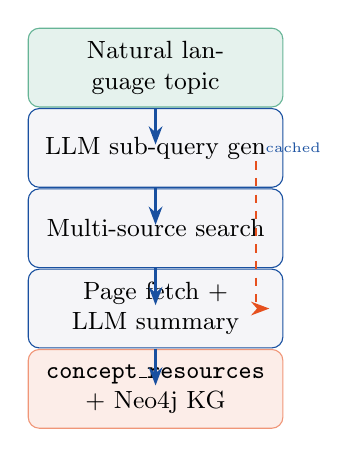
\begin{tikzpicture}[scale=0.85]
        \node[box=3.0cm,fill=codegreen!10,draw=codegreen!60]
          at (0,3.6) {Natural language topic};
        \node[box=3.0cm] at (0,2.4) {LLM sub-query gen};
        \node[box=3.0cm] at (0,1.2) {Multi-source search};
        \node[box=3.0cm] at (0,0.0) {Page fetch + LLM summary};
        \node[box=3.0cm,fill=accent!10,draw=accent!60]
          at (0,-1.2) {\texttt{concept\_resources}\\+ Neo4j KG};

        \foreach \y in {3.0,1.8,0.6,-0.6}
          \draw[arrow] (0,\y) -- (0,{\y-0.55});

        \node[font=\tiny,primary,right] at (1.5,2.4) {cached};
        \draw[dbarrow] (1.5,2.2) -- (1.5,0) -- (1.7,0);
      \end{tikzpicture}
  \end{columns}
\end{frame}

% ── Diagnostic quiz ──────────────────────────────────────────
\begin{frame}{Stage 2 — Diagnostic Assessment \texttt{GET /assess}}
  \begin{columns}
    \column{0.48\textwidth}
      \begin{block}{Question Generation}
        \begin{itemize}\small
          \item 6 MCQ questions per topic
          \item Stratified by difficulty:\\
            \quad 2 \textcolor{codegreen}{\textbf{basic}} (factual recall)\\
            \quad 2 \textcolor{codeorange}{\textbf{intermediate}} (conceptual)\\
            \quad 2 \textcolor{accent}{\textbf{advanced}} (application)
          \item If KG resources exist $\to$ questions grounded in stored summaries
          \item Hardcoded fallback ensures no 500 errors
        \end{itemize}
      \end{block}
    \column{0.50\textwidth}
      \begin{block}{Level Determination \texttt{POST /assess/evaluate}}
        \begin{align*}
          \text{score} &= \frac{\text{correct}}{N} \times 100 \\[4pt]
          \text{level} &= \begin{cases}
            \text{beginner}     & \text{score} < 40 \\
            \text{intermediate} & 40 \le \text{score} \le 70 \\
            \text{advanced}     & \text{score} > 70
          \end{cases}
        \end{align*}
        \vspace{4pt}
        LLM also provides \textbf{personalised feedback} and
        identifies \textbf{weak concept areas} for the roadmap.
      \end{block}
  \end{columns}
\end{frame}

% ── Find gaps ────────────────────────────────────────────────
\begin{frame}{Stage 3 — Gap Analysis \texttt{POST /find-gaps}}
  \begin{center}
  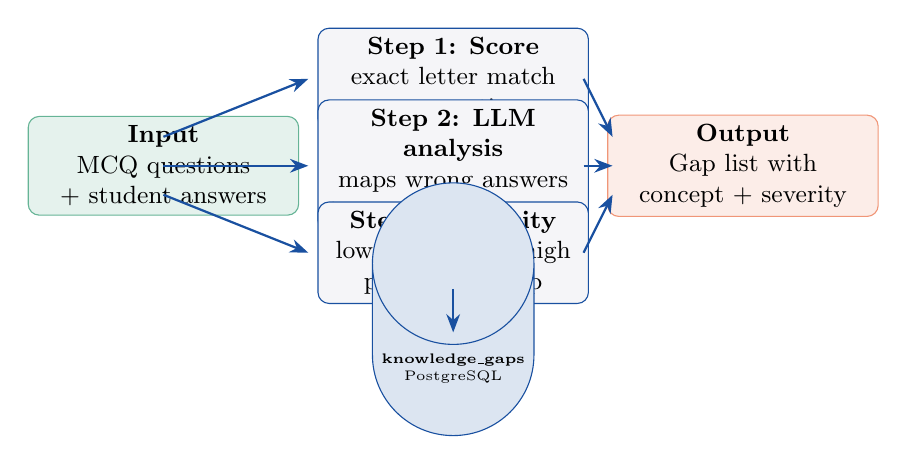
\begin{tikzpicture}[scale=0.92]

    % Input
    \node[box=3.2cm,fill=codegreen!10,draw=codegreen!60] at (-4,0)
        {\textbf{Input}\\MCQ questions\\+ student answers};

    % Step 1
    \node[box=3.2cm] at (0,1.2)
        {\textbf{Step 1: Score}\\exact letter match\\per question};

    % Step 2
    \node[box=3.2cm] at (0,0.0)
        {\textbf{Step 2: LLM analysis}\\maps wrong answers\\to concept weaknesses};

    % Step 3
    \node[box=3.2cm] at (0,-1.2)
        {\textbf{Step 3: Severity}\\low / medium / high\\per concept gap};

    % Output
    \node[box=3.2cm,fill=accent!10,draw=accent!60] at (4,0)
        {\textbf{Output}\\Gap list with\\concept + severity};

    % Persist
    \node[db] at (0,-2.8)
        {\textbf{knowledge\_gaps}\\PostgreSQL};

    \draw[arrow] (-4,0.4) -- (-2.0,1.2);
    \draw[arrow] (-4,0.0) -- (-2.0,0.0);
    \draw[arrow] (-4,-0.4) -- (-2.0,-1.2);
    \draw[arrow] (1.8,1.2) -- (2.2,0.4);
    \draw[arrow] (1.8,0.0) -- (2.2,0.0);
    \draw[arrow] (1.8,-1.2) -- (2.2,-0.4);
    \draw[arrow] (0,-1.7) -- (0,-2.3);

  \end{tikzpicture}
  \end{center}
\end{frame}

% ============================================================
\section{Knowledge Graph \& Database Schema}
% ============================================================

\begin{frame}{Database Schema — PostgreSQL}
  \begin{center}\small
  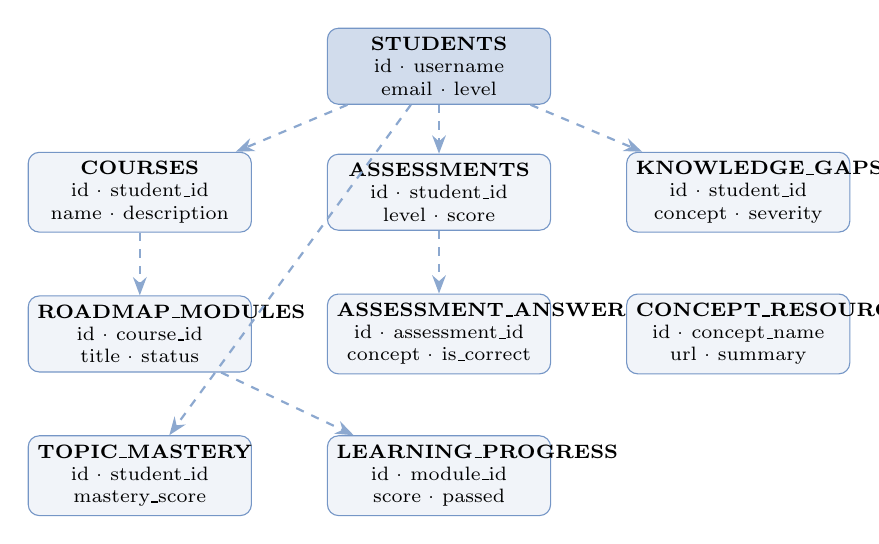
\begin{tikzpicture}[
      table/.style={rectangle,draw=primary!60,fill=primary!6,
                    rounded corners=4pt,text width=2.6cm,
                    align=center,minimum height=0.8cm,font=\scriptsize},
      fk/.style={-Stealth,thick,primary!50,dashed},
    ]

    \node[table,fill=primary!20] (students)  at (0,3.2)   {\textbf{STUDENTS}\\id · username\\email · level};
    \node[table] (courses)   at (-3.8,1.6)   {\textbf{COURSES}\\id · student\_id\\name · description};
    \node[table] (assess)    at (0,1.6)       {\textbf{ASSESSMENTS}\\id · student\_id\\level · score};
    \node[table] (gaps)      at (3.8,1.6)     {\textbf{KNOWLEDGE\_GAPS}\\id · student\_id\\concept · severity};
    \node[table] (answers)   at (0,-0.2)      {\textbf{ASSESSMENT\_ANSWERS}\\id · assessment\_id\\concept · is\_correct};
    \node[table] (roadmap)   at (-3.8,-0.2)   {\textbf{ROADMAP\_MODULES}\\id · course\_id\\title · status};
    \node[table] (mastery)   at (-3.8,-2.0)   {\textbf{TOPIC\_MASTERY}\\id · student\_id\\mastery\_score};
    \node[table] (resources) at (3.8,-0.2)    {\textbf{CONCEPT\_RESOURCES}\\id · concept\_name\\url · summary};
    \node[table] (progress)  at (0,-2.0)      {\textbf{LEARNING\_PROGRESS}\\id · module\_id\\score · passed};

    % FKs
    \foreach \t in {courses,assess,gaps,mastery}
      \draw[fk] (students) -- (\t);
    \draw[fk] (assess)  -- (answers);
    \draw[fk] (roadmap) -- (progress);
    \draw[fk] (courses) -- (roadmap);

  \end{tikzpicture}
  \end{center}
\end{frame}

\begin{frame}{Knowledge Graph — Neo4j}
  \begin{columns}
    \column{0.52\textwidth}
      \begin{tikzpicture}[scale=0.85]
        % Nodes
        \node[circle,draw=primary,fill=primary!20,
              font=\scriptsize,minimum size=1.2cm] (topic) at (0,3)
              {\faBook\\Topic};
        \node[circle,draw=accent,fill=accent!15,
              font=\scriptsize,minimum size=1.0cm] (lg) at (-2,1.5)
              {Level\\Group};
        \node[circle,draw=codegreen!70,fill=codegreen!15,
              font=\scriptsize,minimum size=1.0cm] (mod) at (0,1.5)
              {Module};
        \node[circle,draw=codeorange,fill=codeorange!15,
              font=\scriptsize,minimum size=1.0cm] (concept) at (2,0)
              {Concept};
        \node[circle,draw=darkgray!60,fill=darkgray!10,
              font=\scriptsize,minimum size=1.0cm] (res) at (-2,0)
              {Resource};

        % Edges
        \draw[-Stealth,thick,primary!60]
          (topic) -- node[left,font=\tiny]{HAS\_LEVEL} (lg);
        \draw[-Stealth,thick,primary!60]
          (topic) -- node[right,font=\tiny]{HAS\_MODULE} (mod);
        \draw[-Stealth,thick,codegreen!60]
          (lg) -- node[below left,font=\tiny]{HAS\_MODULE} (mod);
        \draw[-Stealth,thick,codeorange!60]
          (mod) -- node[right,font=\tiny]{TEACHES} (concept);
        \draw[-Stealth,thick,darkgray!60]
          (topic) -- node[left,font=\tiny]{HAS\_RESOURCE} (res);
        \draw[-Stealth,thick,dashed,primary!40]
          (mod.west) to[bend right=20]
          node[left,font=\tiny]{PREREQ\_FOR} (mod.south);
      \end{tikzpicture}
    \column{0.46\textwidth}
      \begin{block}{Graph enables}
        \begin{itemize}\small
          \item \textbf{Prerequisite checking}: hard filter before recommendation
          \item \textbf{Concept coverage}: count concepts per module
          \item \textbf{Weak-concept remediation}: match student gaps to module concepts
          \item \textbf{Path planning}: topological ordering of modules
          \item \textbf{Resource linking}: articles + videos tied to topics
        \end{itemize}
      \end{block}
      \begin{alertblock}{Cypher scoring formula}
        \[\texttt{score} = C_t \times 1.0 + C_w \times 2.0\]
        \footnotesize $C_t$ = concepts taught,\; $C_w$ = weak-concept matches
      \end{alertblock}
  \end{columns}
\end{frame}

% ============================================================
\section{Recommendation System}
% ============================================================

\begin{frame}{Recommendation System — Overview}
  \begin{center}
  \begin{tikzpicture}[
      rec/.style={rectangle,rounded corners=6pt,
                  text width=2.8cm,minimum height=1.0cm,
                  align=center,font=\small},
    ]

    \node[rec,draw=primary,fill=primary!10] (r1) at (0,0)
        {\faProjectDiagram\\\textbf{Rec 1}\\Next Module};
    \node[rec,draw=accent,fill=accent!10] (r2) at (5.5,0)
        {\faStar\\\textbf{Rec 2}\\Gap Resources};

    \node[font=\footnotesize,primary,align=center] at (0,-1.3)
        {\texttt{POST /recommend/next}\\3-stage pipeline};
    \node[font=\footnotesize,accent,align=center] at (5.5,-1.3)
        {\texttt{GET /recommender}\\LLM-ranked resources};

    % Stage boxes for Rec 1
    \foreach \y/\c/\l in {1.8/primary!8/Graph traversal,
                           0.9/primary!15/Weakness scoring,
                           0.0/primary!22/LLM re-ranking}{
      \node[rectangle,rounded corners=3pt,draw=primary!50,
            fill=\c,minimum width=3.2cm,minimum height=0.5cm,
            font=\tiny,align=center] at (-3.5,\y-0.7) {\l};
    }
    \draw[arrow,primary!50] (-3.5,1.35) -- (-3.5,1.05);
    \draw[arrow,primary!50] (-3.5,0.45) -- (-3.5,0.15);

    % Stage boxes for Rec 2
    \foreach \y/\c/\l in {1.8/accent!8/concept\_resources cache,
                           0.9/accent!15/Web + YouTube search,
                           0.0/accent!22/LLM ranking + reasons}{
      \node[rectangle,rounded corners=3pt,draw=accent!50,
            fill=\c,minimum width=3.2cm,minimum height=0.5cm,
            font=\tiny,align=center] at (9.0,\y-0.7) {\l};
    }
    \draw[arrow,accent!50] (9.0,1.35) -- (9.0,1.05);
    \draw[arrow,accent!50] (9.0,0.45) -- (9.0,0.15);

    \draw[arrow] (-1.9,0) -- (r1);
    \draw[arrow] (r2) -- (7.4,0);

  \end{tikzpicture}
  \end{center}
\end{frame}

% ── Rec 1 detail ─────────────────────────────────────────────
\begin{frame}{Recommender 1 — Next Module \texttt{POST /recommend/next}}
  \begin{columns}
    \column{0.5\textwidth}
      \textbf{Stage 1: Graph-aware filtering (Neo4j)}
      \begin{itemize}\small
        \item Find all modules where \textbf{every prerequisite} has been completed
        \item Compute composite score per candidate:
      \end{itemize}
      \vspace{-4pt}
      \[\text{graph\_score} = C_t \cdot 1 + C_w \cdot 2\]
      \vspace{-6pt}
      \begin{itemize}\small
        \item $C_t$: total concepts taught (breadth)
        \item $C_w$: concepts matching student's weak areas (\textbf{weighted ×2})
      \end{itemize}

      \vspace{6pt}
      \textbf{Stage 2: History loading (PostgreSQL)}
      \begin{itemize}\small
        \item Load \texttt{session\_progress}: scores + time per module
        \item Modules with score $<60\%$ $\to$ their concepts become \texttt{weak\_concepts}
      \end{itemize}
    \column{0.48\textwidth}
      \textbf{Stage 3: LLM re-ranking}
      \vspace{4pt}

      The LLM receives:
      \begin{itemize}\footnotesize
        \item Learner level + content preference
        \item Completed module list with scores
        \item Weak concept list
        \item Top 5 graph candidates with scores
      \end{itemize}
      And returns:
      \begin{itemize}\footnotesize
        \item \texttt{recommended\_uid}
        \item \texttt{reason} — 2–3 sentence personalised explanation
        \item \texttt{learning\_tip} — concrete study advice
      \end{itemize}

      \begin{alertblock}{\footnotesize Why 2-stage?}
        \footnotesize Graph ensures \textbf{structural correctness};
        LLM adds \textbf{personalisation}. Neither alone suffices.
      \end{alertblock}
  \end{columns}
\end{frame}

% ── Rec 2 detail ─────────────────────────────────────────────
\begin{frame}{Recommender 2 — Gap Resources \texttt{GET /recommender}}
  \begin{center}
  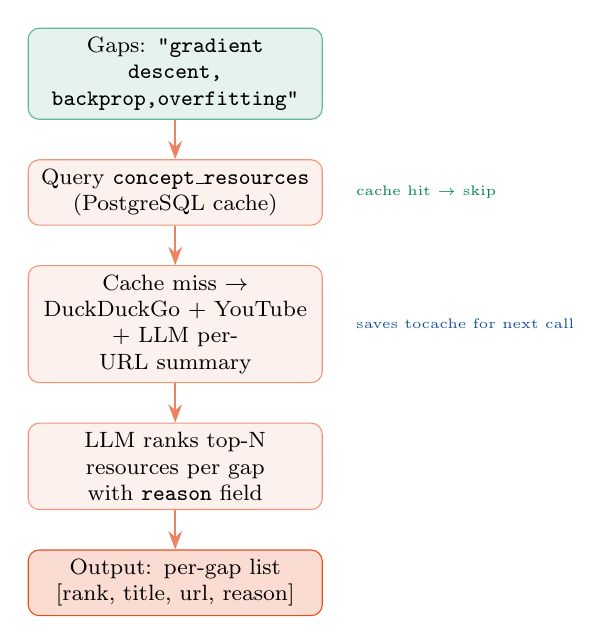
\begin{tikzpicture}[
      node distance=0.3cm,
      stage/.style={rectangle,rounded corners=4pt,draw=accent!60,
                    fill=accent!8,text width=3.5cm,
                    minimum height=0.7cm,align=center,font=\footnotesize},
    ]

    \node[stage,fill=codegreen!10,draw=codegreen!60] (in)
        {Gaps: \texttt{"gradient descent,\\backprop,overfitting"}};

    \node[stage,below=0.5cm of in] (cache)
        {Query \texttt{concept\_resources}\\(PostgreSQL cache)};

    \node[stage,below=0.5cm of cache] (miss)
        {Cache miss $\to$\\DuckDuckGo + YouTube\\+ LLM per-URL summary};

    \node[stage,below=0.5cm of miss] (rank)
        {LLM ranks top-N\\resources per gap\\with \texttt{reason} field};

    \node[stage,fill=accent!20,draw=accent,below=0.5cm of rank] (out)
        {Output: per-gap list\\$[$rank, title, url, reason$]$};

    \foreach \a/\b in {in/cache,cache/miss,miss/rank,rank/out}
      \draw[arrow,accent!70] (\a) -- (\b);

    \node[font=\tiny,primary,right=0.3cm of cache]
        {\textcolor{codegreen}{cache hit $\to$ skip}};
    \node[font=\tiny,primary,right=0.3cm of miss]
        {saves to\\cache for next call};

  \end{tikzpicture}
  \end{center}
\end{frame}

% ── Scoring formula ──────────────────────────────────────────
\begin{frame}{Module Scoring Formula}
  \begin{columns}
    \column{0.55\textwidth}
      \begin{block}{Graph score (Neo4j Cypher)}
        \[
          S_{\text{graph}}(m) = C_t(m) \cdot w_1 + C_w(m) \cdot w_2
        \]
        where:
        \begin{align*}
          C_t(m) &= |\{c \in \text{Concepts}(m)\}| \\
          C_w(m) &= |\{c \in \text{Concepts}(m) \cap W\}| \\
          W      &= \text{student weak concept set} \\
          w_1    &= 1.0 \quad \text{(breadth)} \\
          w_2    &= 2.0 \quad \text{(remediation priority)}
        \end{align*}
      \end{block}
    \column{0.43\textwidth}
      \begin{block}{Weak concept derivation}
        \small
        A concept $c$ enters $W$ when:
        \begin{enumerate}
          \item Module quiz score $< 60\%$
          \item AND module teaches concept $c$
        \end{enumerate}
        \vspace{4pt}
        Or directly from \texttt{/find-gaps}:\\
        wrong answer $\to$ LLM $\to$ concept name $\to$ $W$
      \end{block}
      \vspace{6pt}
      \begin{alertblock}{Key insight}
        \small Prerequisite satisfaction is a \textbf{hard filter}, not a score component — structural correctness is non-negotiable.
      \end{alertblock}
  \end{columns}
\end{frame}

% ============================================================
\section{API Design}
% ============================================================

\begin{frame}{API Endpoints — Full Reference}
  \begin{columns}
    \column{0.5\textwidth}
      \begin{table}\footnotesize
        \begin{tabular}{lp{4.2cm}}
          \toprule
          \textbf{Endpoint} & \textbf{Purpose} \\
          \midrule
          \texttt{POST /students}         & Register student \\
          \texttt{POST /students/\{id\}/verify} & Email verification \\
          \texttt{POST /deep-search}      & Multi-source search + summarise \\
          \texttt{GET  /assess}           & Generate diagnostic quiz \\
          \texttt{POST /assess/evaluate}  & Score + determine level \\
          \texttt{POST /find-gaps}        & Identify knowledge gaps \\
          \texttt{GET  /roadmap}          & Build N-level roadmap \\
          \texttt{GET  /lesson}           & Generate lesson content \\
          \texttt{POST /quiz}             & Generate module quiz \\
          \bottomrule
        \end{tabular}
      \end{table}
    \column{0.5\textwidth}
      \begin{table}\footnotesize
        \begin{tabular}{lp{4.2cm}}
          \toprule
          \textbf{Endpoint} & \textbf{Purpose} \\
          \midrule
          \texttt{GET  /recommender}      & Rank resources per gap \\
          \texttt{POST /recommend/next}   & Next module recommendation \\
          \texttt{POST /next}             & Advance session, get next lesson \\
          \texttt{POST /session/start}    & Create learning session \\
          \texttt{GET  /resources}        & Query Neo4j for topic resources \\
          \texttt{GET  /knowledge}        & Open knowledge DBs lookup \\
          \texttt{GET  /users/\{id\}/history} & Full learning history \\
          \texttt{GET  /deepSearch}       & Streaming deep search \\
          \bottomrule
        \end{tabular}
      \end{table}
  \end{columns}
\end{frame}

% ============================================================
\section{Caching \& Performance}
% ============================================================

\begin{frame}{Caching Strategy}
  \begin{center}
  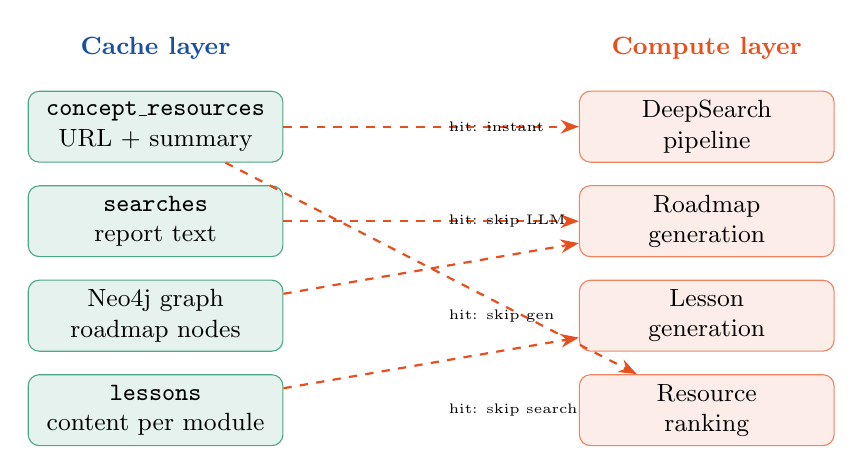
\begin{tikzpicture}[
      cache/.style={rectangle,rounded corners=4pt,draw=codegreen!70,
                    fill=codegreen!10,text width=3.0cm,
                    minimum height=0.9cm,align=center,font=\small},
      miss/.style={rectangle,rounded corners=4pt,draw=accent!70,
                   fill=accent!10,text width=3.0cm,
                   minimum height=0.9cm,align=center,font=\small},
    ]

    \begin{scope}[yshift=0.5cm]
      \node[font=\small\bfseries,primary] at (-3.5,1.5) {Cache layer};
      \node[font=\small\bfseries,accent]  at (3.5,1.5)  {Compute layer};

      \node[cache] (cr) at (-3.5,0.5)  {\texttt{concept\_resources}\\URL + summary};
      \node[cache] (sr) at (-3.5,-0.7) {\texttt{searches}\\report text};
      \node[cache] (ng) at (-3.5,-1.9) {Neo4j graph\\roadmap nodes};
      \node[cache] (sl) at (-3.5,-3.1) {\texttt{lessons}\\content per module};

      \node[miss] (ds) at (3.5,0.5)  {DeepSearch\\pipeline};
      \node[miss] (rg) at (3.5,-0.7) {Roadmap\\generation};
      \node[miss] (lg) at (3.5,-1.9) {Lesson\\generation};
      \node[miss] (rs) at (3.5,-3.1) {Resource\\ranking};

      \foreach \c/\m in {cr/ds,sr/rg,ng/rg,sl/lg,cr/rs}{
        \draw[dbarrow] (\c) -- (\m);
      }

      \node[font=\tiny,right=0.1cm] at (0,0.5)  {hit: instant};
      \node[font=\tiny,right=0.1cm] at (0,-0.7) {hit: skip LLM};
      \node[font=\tiny,right=0.1cm] at (0,-1.9) {hit: skip gen};
      \node[font=\tiny,right=0.1cm] at (0,-3.1) {hit: skip search};
    \end{scope}
  \end{tikzpicture}
  \end{center}
\end{frame}

% ============================================================
\section{Evaluation}
% ============================================================

% ── Evaluation overview ───────────────────────────────────────
\begin{frame}{Evaluation Strategy — Two Complementary Axes}
  \begin{columns}
    \column{0.5\textwidth}
      \begin{block}{Axis 1 — Benchmark datasets}
        \begin{itemize}\small
          \item Compare PathOptLearn's knowledge-tracing signal
                against three established educational datasets
          \item Metrics: \textbf{AUC}, \textbf{Accuracy}, \textbf{RMSE}
          \item Baseline: Logistic Regression on user history features
        \end{itemize}
        \vspace{4pt}
        {\footnotesize\begin{tabular}{ll}
          \toprule
          Dataset & Scale \\
          \midrule
          Riiid!      & 13M interactions, 1.1M students \\
          EdNet-KT1   & 95M interactions, 784K students \\
          ASSISTments & 278K–708K interactions \\
          \bottomrule
        \end{tabular}}
      \end{block}
    \column{0.48\textwidth}
      \begin{block}{Axis 2 — LLM student simulation}
        \begin{itemize}\small
          \item Synthetic students with configurable profiles
                traverse the full learning flow via the real API
          \item Profiles: beginner · intermediate · advanced ·
                struggling · fast\_learner
          \item Measures: pass rate, retries, gap closure,
                recommendation relevance
        \end{itemize}
      \end{block}
      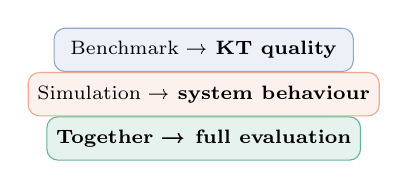
\begin{tikzpicture}[scale=0.75]
        \node[rectangle,rounded corners=4pt,draw=primary!50,
              fill=primary!8,minimum width=3.8cm,
              minimum height=0.55cm,font=\scriptsize,align=center]
          at (0,0) {Benchmark → \textbf{KT quality}};
        \node[rectangle,rounded corners=4pt,draw=accent!50,
              fill=accent!8,minimum width=3.8cm,
              minimum height=0.55cm,font=\scriptsize,align=center]
          at (0,-0.75) {Simulation → \textbf{system behaviour}};
        \node[rectangle,rounded corners=4pt,draw=codegreen!60,
              fill=codegreen!10,minimum width=3.8cm,
              minimum height=0.55cm,font=\scriptsize\bfseries,align=center]
          at (0,-1.5) {Together → full evaluation};
      \end{tikzpicture}
  \end{columns}
\end{frame}

% ── Benchmark protocol ────────────────────────────────────────
\begin{frame}{Benchmark Protocol — Leave-One-Out per Student}
  \begin{center}
  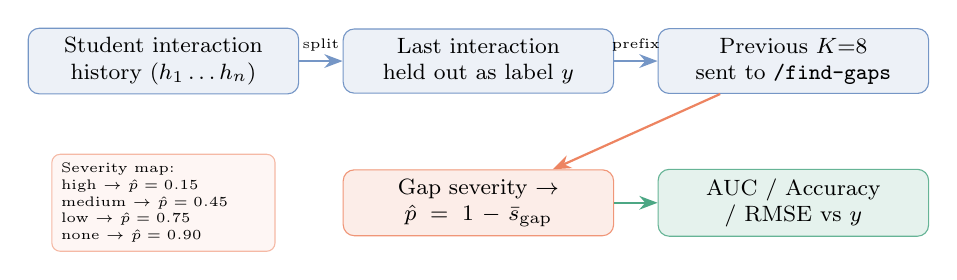
\begin{tikzpicture}[
      bstep/.style={rectangle,rounded corners=4pt,draw=primary!60,
                   fill=primary!8,text width=3.2cm,minimum height=0.8cm,
                   align=center,font=\footnotesize},
    ]
    \node[bstep] (A) at (0,0)    {Student interaction\\history $(h_1 \ldots h_n)$};
    \node[bstep] (B) at (4.0,0)  {Last interaction\\held out as label $y$};
    \node[bstep] (C) at (8.0,0)  {Previous $K{=}8$\\sent to \texttt{/find-gaps}};
    \node[bstep,fill=accent!10,draw=accent!60]
                 (D) at (4.0,-1.8) {Gap severity $\to$\\$\hat{p} = 1 - \bar{s}_{\text{gap}}$};
    \node[bstep,fill=codegreen!10,draw=codegreen!60]
                 (E) at (8.0,-1.8) {AUC / Accuracy\\/ RMSE vs $y$};

    \draw[-Stealth,thick,primary!60] (A) -- (B);
    \draw[-Stealth,thick,primary!60] (B) -- (C);
    \draw[-Stealth,thick,accent!70]  (C) -- (D);
    \draw[-Stealth,thick,codegreen!70] (D) -- (E);

    \node[font=\tiny,above] at ($(A)!0.5!(B)$) {split};
    \node[font=\tiny,above] at ($(B)!0.5!(C)$) {prefix};

    % Severity map
    \node[rectangle,rounded corners=3pt,draw=accent!40,fill=accent!5,
          font=\tiny,align=left,text width=2.6cm]
      at (0,-1.8) {
        Severity map:\\
        high   $\to$ $\hat{p}=0.15$\\
        medium $\to$ $\hat{p}=0.45$\\
        low    $\to$ $\hat{p}=0.75$\\
        none   $\to$ $\hat{p}=0.90$
      };

  \end{tikzpicture}
  \end{center}
  \vspace{4pt}
  \begin{columns}
    \column{0.5\textwidth}
      \centering\footnotesize
      Compared against:\\
      (1) Logistic Regression on student features\\
      (2) Random baseline ($\hat{p} \sim \mathcal{U}(0.4,\,0.6)$)
    \column{0.5\textwidth}
      \centering\footnotesize
      Features used by baseline:\\
      avg\_correct, n\_interactions, avg\_elapsed\_ms,\\
      avg\_hints (ASSISTments), opportunity count
  \end{columns}
\end{frame}

% ── Dataset schemas ───────────────────────────────────────────
\begin{frame}{Benchmark Datasets — Schema Summary}
  \begin{columns}
    \column{0.33\textwidth}
      \textbf{Riiid!}\\[4pt]
      {\scriptsize\begin{tabular}{ll}
        \toprule
        Column & Type \\
        \midrule
        user\_id & int \\
        question\_id & int \\
        answered\_correctly & int8 \\
        timestamp & int64 \\
        elapsed\_time & float \\
        content\_type & int8 \\
        \bottomrule
      \end{tabular}}
      \vspace{4pt}\\
      \scriptsize 13M rows · 1.1M users\\
      10K+ questions · 293 tags\\
      \textbf{Metric:} AUC
    \column{0.33\textwidth}
      \textbf{EdNet-KT1}\\[4pt]
      {\scriptsize\begin{tabular}{ll}
        \toprule
        Column & Type \\
        \midrule
        user\_id & int \\
        question\_id & str \\
        user\_answer & char \\
        correct & int \\
        timestamp & int64 \\
        elapsed\_time & int \\
        \bottomrule
      \end{tabular}}
      \vspace{4pt}\\
      \scriptsize 95M rows · 784K users\\
      13K questions · 188 skills\\
      \textbf{Metric:} AUC / Accuracy
    \column{0.33\textwidth}
      \textbf{ASSISTments}\\[4pt]
      {\scriptsize\begin{tabular}{ll}
        \toprule
        Column & Type \\
        \midrule
        user\_id & int \\
        problem\_id & int \\
        correct & int \\
        hint\_count & int \\
        skill\_name & str \\
        opportunity & int \\
        \bottomrule
      \end{tabular}}
      \vspace{4pt}\\
      \scriptsize 278K–708K rows\\
      4K–20K users · 102 skills\\
      \textbf{Metric:} AUC / RMSE
  \end{columns}
\end{frame}

% ── Expected benchmark results ────────────────────────────────
\begin{frame}{Benchmark Results — Expected Output}
  \begin{columns}
    \column{0.58\textwidth}
      \begin{block}{Result table format (\texttt{results.json})}
        \begin{center}\scriptsize
        \begin{tabular}{llrrr}
          \toprule
          \textbf{Dataset} & \textbf{Model} & \textbf{AUC} & \textbf{Acc} & \textbf{RMSE} \\
          \midrule
          \multirow{3}{*}{Riiid!}
            & PathOptLearn   & -- & -- & -- \\
            & LogReg (base.) & -- & -- & -- \\
            & Random         & {\raise.17ex\hbox{$\scriptstyle\sim$}}0.50 & -- & -- \\
          \midrule
          \multirow{3}{*}{EdNet}
            & PathOptLearn   & -- & -- & -- \\
            & LogReg (base.) & -- & -- & -- \\
            & Random         & {\raise.17ex\hbox{$\scriptstyle\sim$}}0.50 & -- & -- \\
          \midrule
          \multirow{3}{*}{ASSISTments}
            & PathOptLearn   & -- & -- & -- \\
            & LogReg (base.) & -- & -- & -- \\
            & Random         & {\raise.17ex\hbox{$\scriptstyle\sim$}}0.50 & -- & -- \\
          \bottomrule
        \end{tabular}
        \end{center}
      \end{block}
      \vspace{4pt}
      \scriptsize Literature baselines for reference:\\
      Deep KT (DKT): 0.75–0.82 AUC $\cdot$
      LogReg: 0.70–0.75 AUC
    \column{0.40\textwidth}
      \begin{alertblock}{Interpretation}
        \small PathOptLearn is \textbf{not a KT model} —
        it is a learning system. The benchmark measures
        whether its gap-detection signal correlates with
        actual student correctness.\\[6pt]
        AUC $>$ 0.65 indicates the gap severity proxy
        has meaningful predictive power beyond random.
      \end{alertblock}
      \vspace{6pt}
      \begin{block}{Run command}
        \scriptsize
        \texttt{python run\_benchmark.py}\\
        \texttt{\ \ --dataset riiid}\\
        \texttt{\ \ --data train.csv}\\
        \texttt{\ \ --api http://localhost:8000}\\
        \texttt{\ \ --sample 500}\\
        \texttt{\ \ --output results.json}
      \end{block}
  \end{columns}
\end{frame}

% ── LLM simulation ────────────────────────────────────────────
\begin{frame}{LLM User Simulation — Architecture}
  \begin{center}
  \begin{tikzpicture}[
      sbox/.style={rectangle,rounded corners=5pt,draw=primary!60,
                   fill=primary!8,text width=2.6cm,minimum height=0.9cm,
                   align=center,font=\scriptsize},
      pbox/.style={rectangle,rounded corners=4pt,draw=accent!50,
                   fill=accent!8,text width=2.2cm,minimum height=0.7cm,
                   align=center,font=\tiny},
    ]

    % Central student brain
    \node[circle,draw=accent,fill=accent!15,
          font=\small,minimum size=1.6cm,align=center]
      (brain) at (0,0) {\faBrain\\LLM\\student};

    % Profile input
    \node[pbox] (prof) at (-4.5,1.0)
        {Profile:\\beginner / advanced\\struggling \ldots};
    \node[pbox] (mem)  at (-4.5,-1.0)
        {Working memory:\\lesson summaries\\(last 4)};

    % API calls
    \node[sbox] (ds)  at (4.5, 2.4) {DeepSearch\\API};
    \node[sbox] (dq)  at (4.5, 0.8) {Diagnostic\\quiz API};
    \node[sbox] (rm)  at (4.5,-0.8) {Roadmap\\API};
    \node[sbox] (les) at (4.5,-2.4) {Lesson + Quiz\\API};

    % Arrows
    \draw[-Stealth,thick,accent!70] (prof) -- (brain);
    \draw[-Stealth,thick,primary!60] (mem)  -- (brain);
    \draw[Stealth-Stealth,thick,primary!40] (brain) -- (ds);
    \draw[Stealth-Stealth,thick,primary!40] (brain) -- (dq);
    \draw[Stealth-Stealth,thick,primary!40] (brain) -- (rm);
    \draw[Stealth-Stealth,thick,primary!40] (brain) -- (les);

    % Log output
    \node[rectangle,rounded corners=4pt,draw=codegreen!60,
          fill=codegreen!10,font=\scriptsize,minimum width=3.0cm,
          minimum height=0.6cm,align=center]
      (log) at (0,-2.4) {simulation\_log.jsonl};
    \draw[-Stealth,thick,codegreen!70] (brain) -- (log);

    \node[font=\tiny,left=0.2cm of log] {events:};

  \end{tikzpicture}
  \end{center}
\end{frame}

% ── Simulation profiles ───────────────────────────────────────
\begin{frame}{LLM Simulation — Student Profiles \& Metrics}
  \begin{columns}
    \column{0.52\textwidth}
      \begin{block}{Five student profiles}
        \begin{center}\scriptsize
        \begin{tabular}{lccc}
          \toprule
          \textbf{Profile} & \textbf{Error rate} & \textbf{Attention} & \textbf{Patience} \\
          \midrule
          beginner     & 65\% & low    & 2 retries \\
          intermediate & 35\% & medium & 3 retries \\
          advanced     & 10\% & high   & 2 retries \\
          struggling   & 75\% & high   & 4 retries \\
          fast\_learner & 15\% & high   & 1 retry   \\
          \bottomrule
        \end{tabular}
        \end{center}
        \vspace{4pt}
        \scriptsize
        The LLM answers each MCQ \textbf{in character}:
        it receives the question + its working memory + profile
        as system prompt, then picks a letter A–D.
      \end{block}
    \column{0.46\textwidth}
      \begin{block}{Metrics collected per run}
        \begin{itemize}\small
          \item \textbf{Diagnostic score} and assigned level
          \item \textbf{Per-module}: score, attempts, gaps found
          \item \textbf{Pass rate} across all modules
          \item \textbf{Total retries} (measure of recommendation quality)
          \item \textbf{Gap closure}: were gaps from diagnosis resolved?
          \item \textbf{Event log}: full JSONL trace for analysis
        \end{itemize}
      \end{block}
      \vspace{4pt}
      % Bar chart: expected pass rate per profile
      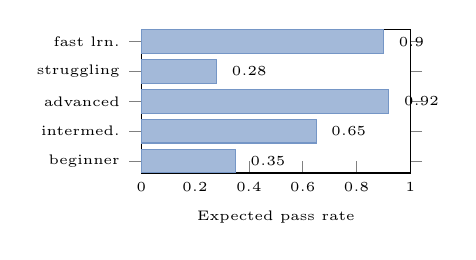
\begin{tikzpicture}
        \begin{axis}[
          width=5.0cm, height=3.4cm,
          xbar, xmin=0, xmax=1,
          ytick=data,
          yticklabels={beginner,intermed.,advanced,struggling,fast lrn.},
          yticklabel style={font=\tiny},
          xticklabel style={font=\tiny},
          xlabel style={font=\tiny},
          xlabel={Expected pass rate},
          bar width=0.3cm,
          nodes near coords,
          nodes near coords style={font=\tiny,xshift=2pt},
        ]
          \addplot[fill=primary!40,draw=primary!60] coordinates {
            (0.35,0) (0.65,1) (0.92,2) (0.28,3) (0.90,4)
          };
        \end{axis}
      \end{tikzpicture}
  \end{columns}
\end{frame}

% ── Simulation flow ───────────────────────────────────────────
\begin{frame}{LLM Simulation — Full Flow Exercised}
  \begin{center}\small
  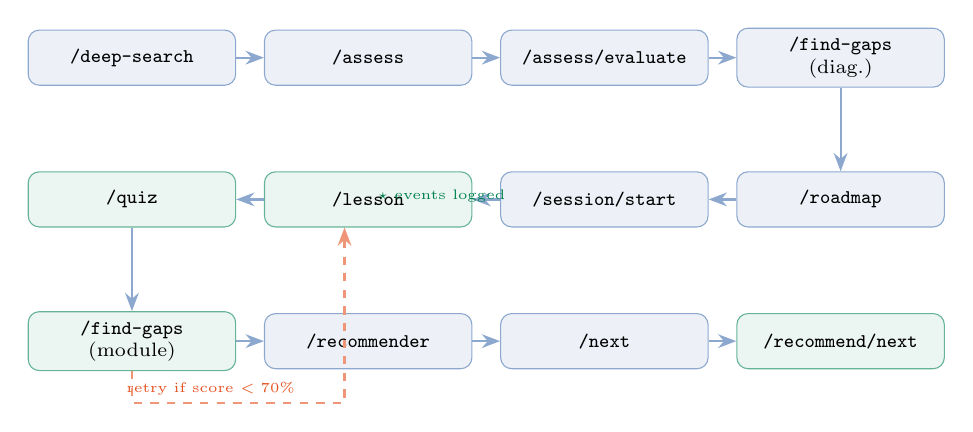
\begin{tikzpicture}[
      ev/.style={rectangle,rounded corners=4pt,draw=primary!50,
                 fill=primary!8,text width=2.4cm,minimum height=0.7cm,
                 align=center,font=\scriptsize},
      logged/.style={ev,draw=codegreen!60,fill=codegreen!8},
    ]

    \node[ev]     (ds)   at (0,0)      {\texttt{/deep-search}};
    \node[ev]     (dq)   at (3.0,0)    {\texttt{/assess}};
    \node[ev]     (eval) at (6.0,0)    {\texttt{/assess/evaluate}};
    \node[ev]     (fg1)  at (9.0,0)    {\texttt{/find-gaps}\\(diag.)};
    \node[ev]     (rm)   at (9.0,-1.8) {\texttt{/roadmap}};
    \node[ev]     (ss)   at (6.0,-1.8) {\texttt{/session/start}};
    \node[logged] (les)  at (3.0,-1.8) {\texttt{/lesson}};
    \node[logged] (qz)   at (0,-1.8)   {\texttt{/quiz}};
    \node[logged] (fg2)  at (0,-3.6)   {\texttt{/find-gaps}\\(module)};
    \node[ev]     (rec)  at (3.0,-3.6) {\texttt{/recommender}};
    \node[ev]     (nxt)  at (6.0,-3.6) {\texttt{/next}};
    \node[logged] (rn)   at (9.0,-3.6) {\texttt{/recommend/next}};

    \foreach \a/\b in {ds/dq,dq/eval,eval/fg1,fg1/rm,rm/ss,ss/les,
                        les/qz,qz/fg2,fg2/rec,rec/nxt,nxt/rn}
      \draw[-Stealth,thick,primary!50] (\a) -- (\b);

    % Retry loop
    \draw[-Stealth,dashed,accent!60,thick]
      (fg2.south) -- ++(0,-0.4) -| ([xshift=-0.3cm]les.south);
    \node[font=\tiny,accent] at (1.0,-4.2) {retry if score $<70$\%};

    \node[font=\tiny,codegreen,below right] at (3.0,-1.55)
        {$\star$ events logged};

  \end{tikzpicture}
  \end{center}
\end{frame}

% ── Run commands ─────────────────────────────────────────────
\begin{frame}{Running the Evaluation}
  \begin{columns}
    \column{0.5\textwidth}
      \begin{block}{Benchmark}
        \scriptsize
        \texttt{\# Install dependencies}\\
        \texttt{pip install -r evalution/requirements.txt}\\[6pt]
        \texttt{\# Riiid!}\\
        \texttt{python run\_benchmark.py \textbackslash}\\
        \texttt{\ \ --dataset riiid \textbackslash}\\
        \texttt{\ \ --data path/to/train.csv \textbackslash}\\
        \texttt{\ \ --sample 500 --output riiid.json}\\[6pt]
        \texttt{\# EdNet-KT1 (per-student dir)}\\
        \texttt{python run\_benchmark.py \textbackslash}\\
        \texttt{\ \ --dataset ednet \textbackslash}\\
        \texttt{\ \ --data path/to/KT1/ \textbackslash}\\
        \texttt{\ \ --topic "TOEIC English"}\\[6pt]
        \texttt{\# ASSISTments}\\
        \texttt{python run\_benchmark.py \textbackslash}\\
        \texttt{\ \ --dataset assist \textbackslash}\\
        \texttt{\ \ --data skill\_builder\_data.csv}
      \end{block}
    \column{0.48\textwidth}
      \begin{block}{User simulation}
        \scriptsize
        \texttt{\# Single beginner}\\
        \texttt{python llm\_student.py \textbackslash}\\
        \texttt{\ \ --topic "Machine Learning" \textbackslash}\\
        \texttt{\ \ --profiles beginner}\\[6pt]
        \texttt{\# All 5 profiles in parallel}\\
        \texttt{python llm\_student.py \textbackslash}\\
        \texttt{\ \ --topic "Machine Learning" \textbackslash}\\
        \texttt{\ \ --profiles beginner intermediate}\\
        \texttt{\ \ \ \ advanced struggling fast\_learner}\\
        \texttt{\ \ --output sim\_log.jsonl}\\[6pt]
        \texttt{\# With prior knowledge context}\\
        \texttt{python llm\_student.py \textbackslash}\\
        \texttt{\ \ --history "I know linear algebra" \textbackslash}\\
        \texttt{\ \ --profiles intermediate}
      \end{block}
  \end{columns}
\end{frame}

% ============================================================
\section{Contributions \& Conclusion}
% ============================================================

\begin{frame}{Research Contributions}
  \begin{columns}
    \column{0.5\textwidth}
      \begin{block}{Technical contributions}
        \begin{enumerate}\small
          \item \textbf{Knowledge-graph-grounded quiz generation}:
                questions based on stored, verified summaries — not hallucinations
          \item \textbf{Hybrid recommendation}:
                graph traversal (structural) + LLM re-ranking (personal)
          \item \textbf{Persistent gap tracking}:
                concept-level weakness accumulates across sessions
          \item \textbf{Per-URL summarisation pipeline}:
                every resource has an LLM summary focused on the target concept
        \end{enumerate}
      \end{block}
    \column{0.48\textwidth}
      \begin{block}{System properties}
        \begin{itemize}\small
          \item \textcolor{codegreen}{\faCheck}\ Fully offline (Ollama, no external API keys)
          \item \textcolor{codegreen}{\faCheck}\ Cache-first design (no redundant LLM calls)
          \item \textcolor{codegreen}{\faCheck}\ Fallback chains at every LLM call
          \item \textcolor{codegreen}{\faCheck}\ Dual-database: relational + graph
          \item \textcolor{codegreen}{\faCheck}\ Containerised (one command deploy)
        \end{itemize}
      \end{block}
      \begin{alertblock}{Open directions}
        \begin{itemize}\footnotesize
          \item Collaborative filtering across students
          \item Spaced repetition scheduling
          \item Multi-modal resources (PDF, slides)
          \item Evaluation against human tutors
        \end{itemize}
      \end{alertblock}
  \end{columns}
\end{frame}

\begin{frame}{Conclusion}
  \begin{center}
  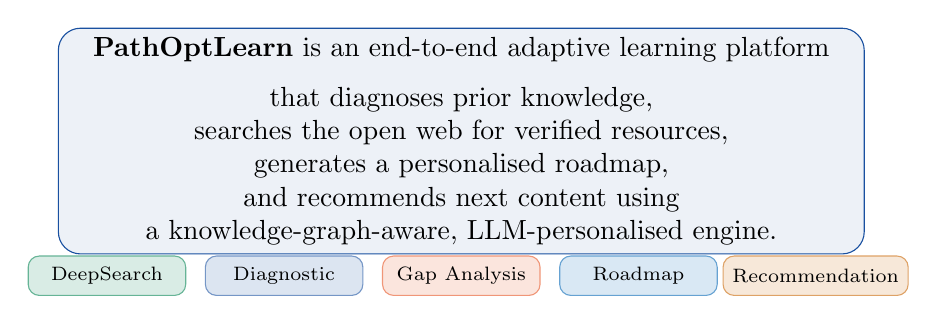
\begin{tikzpicture}[scale=0.9]
    \node[rectangle,rounded corners=8pt,draw=primary,
          fill=primary!8,text width=10cm,
          minimum height=2.5cm,align=center,font=\normalsize]
      at (0,0) {
        \textbf{PathOptLearn} is an end-to-end adaptive learning platform\\[6pt]
        that \alert{diagnoses} prior knowledge,\\
        \alert{searches} the open web for verified resources,\\
        \alert{generates} a personalised roadmap,\\
        and \alert{recommends} next content using\\
        a knowledge-graph-aware, LLM-personalised engine.
      };

    \foreach \i/\l/\c in {
        0/DeepSearch/codegreen,
        1/Diagnostic/primary,
        2/Gap Analysis/accent,
        3/Roadmap/codeblue,
        4/Recommendation/codeorange}{
      \node[rectangle,rounded corners=4pt,draw=\c!60,fill=\c!15,
            minimum width=2.0cm,minimum height=0.5cm,
            font=\scriptsize,align=center]
        at ({(\i-2)*2.5},-1.9) {\l};
    }
  \end{tikzpicture}
  \end{center}
  \vspace{8pt}
  \begin{center}
    \large\textbf{Thank you}\\[4pt]
    \normalsize Source: \texttt{github.com/moujar/PathOptLearn}\\[4pt]
    \footnotesize Questions?
  \end{center}
\end{frame}

% ============================================================
\end{document}
